\chapter{Kravspecifikation}
I dette kapitel vil de forskellige krav for systemet blive gennemgået. Disse krav er blevet lavet ud fra problemformuleringen og MoSCoW'en fra det forrige kapitel. Først bliver de forskellige aktører for applikationen præsenteret, hvorefter user stories præsenteres.
\section{Aktør-kontekst}

Applikationen har 3 forskellige aktører, 2 primære og 1 sekunder, som kan ses herunder på figur \ref{fig:aktor_konteks}.
\begin{figure}[h]
  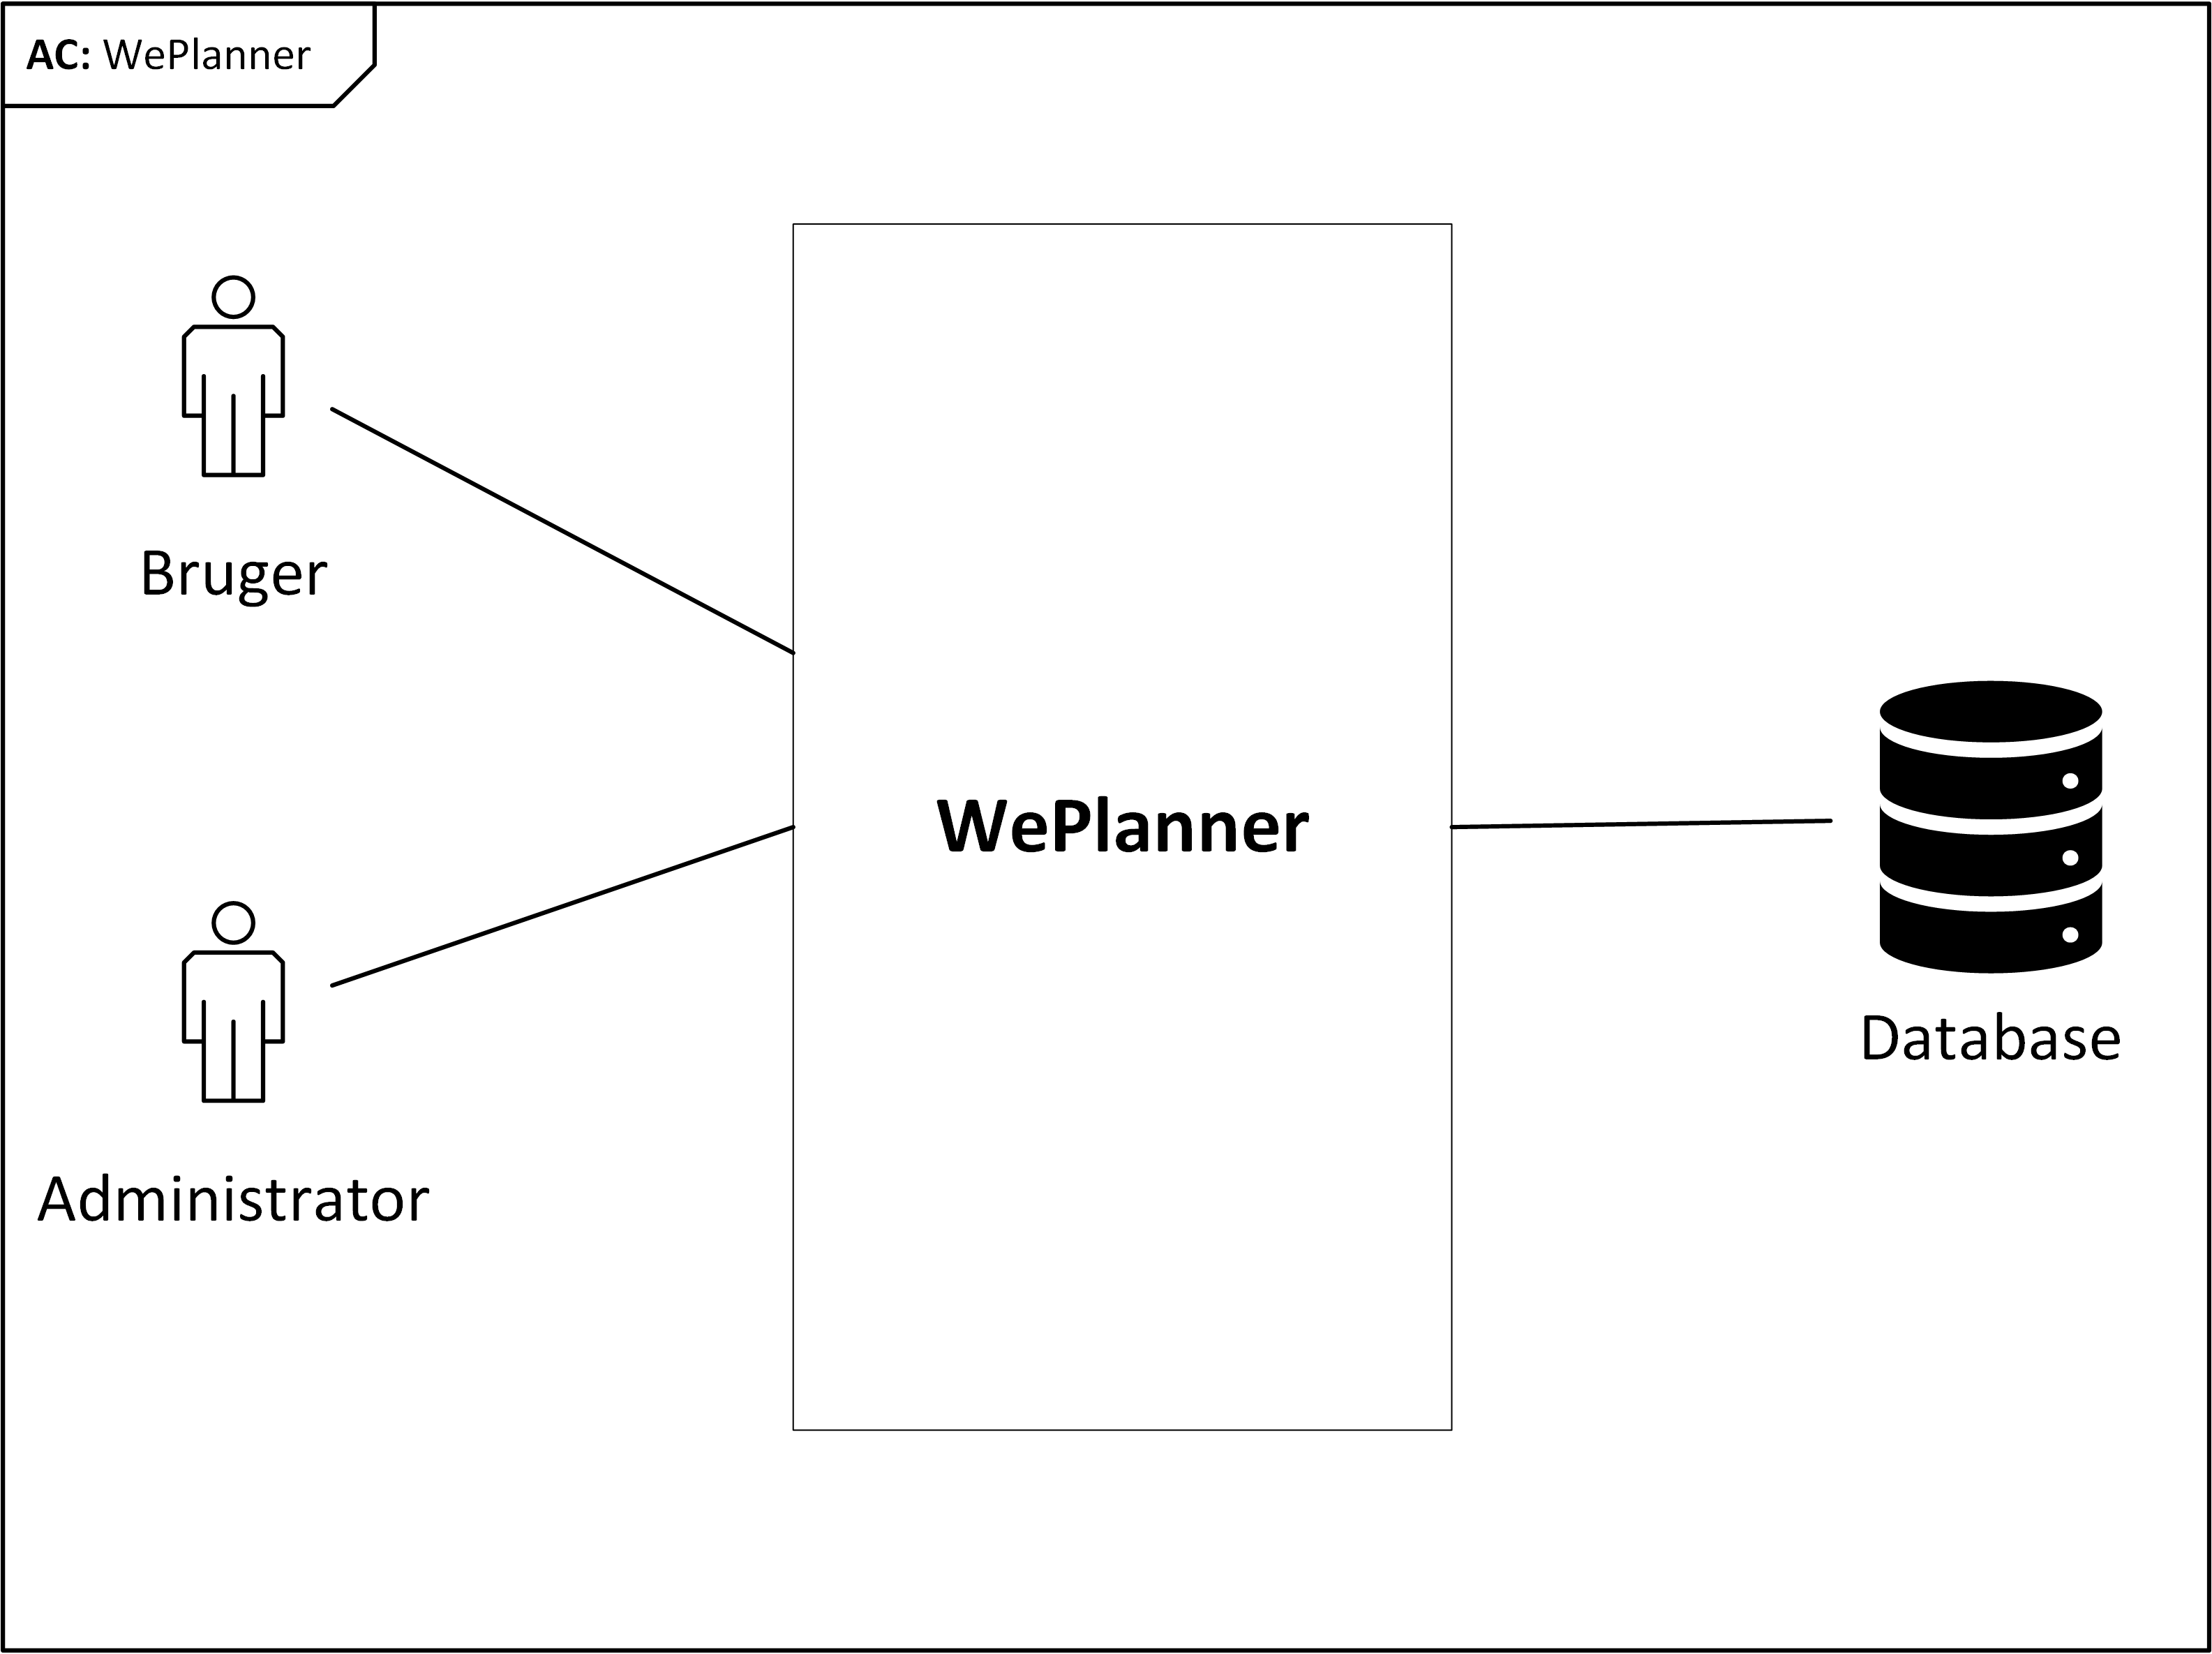
\includegraphics[width=\linewidth]{Kravspecifikation/Images/Aktor-kontekst_diagram.png}
  \caption{Aktør-kontekst diagram}
  \label{fig:aktor_konteks}
\end{figure}

\subsection{Bruger:}
Aktøren bruger er en person som har oprettet et brugerlogin til WePlanner, og dermed kan logge sig ind på siden. En bruger kan være en del af et eller flere bofællesskaber, og bliver en del af et sådant fællesskab, enten ved selv at oprette et fællesskab, eller ved at blive inviteret til et. Når en bruger er en del af fællesskabet kan brugeren se og oprette widgets på siden, som alle medlemmer af gruppen er en del af. 

\subsection{Administrator:}
I hvert bofællesskab vil der være en eller flere administratorer. Brugeren som opretter et bofællesskab vil automatisk blive administrator. En administrator kan derefter ophøje et andet medlem af gruppens rettigheder til administratorrettigheder. \\
En administrator har rettighed til at smide brugere ud af et bofællesskab, samt slette oprettede widgets.

\subsection{Database:}
Databasen er SQL-baseret, og indeholder informationerne for alle brugere og bofællesskaber. Det er her der bliver gemt loginoplysninger for brugere, og også her alle widgets for de individuelle bofællesskaber vil blive gemt. Databasen vil ligge online.
\section{User stories}
For at definere hvilke funktioner applikationen og dens widgets skal indeholde, udarbejdes en user-story for hver funktion som en bruger/administrator skal kunne udføre. På denne måde sættes funktionerne i perspektiv i forhold til resten af applikationen. User-stories gør desuden at vi ikke fastlægger os på specifikke design-beslutninger allerede i en UC, men i stedet udvikler disse iterativt under design- og implementerings- fasen. 


\subsection{Indstillinger og almindelige operationer}
Dette afsnit indeholder user-stories der beskriver indstillinger for en bruger samt en gruppe. Disse indstillinger kan bruges til at personliggøre gruppen/profilen samt udføre nødvendige handlinger, som fx. at fjerne/tilføje brugere fra en gruppe.
\subsubsection{Bruger Operationer}

\noindent User stories for operationer (bruger)\newline

\begin{tabular}{p{2.5in}p{2.5in}}
\textbf{\underline{Opret bruger}}\newline \textbf{Som} bruger\newline \textbf{Vil jeg} gerne kunne oprette mig som bruger til webappliaktionen med email og adgangskode\newline \textbf{For at} kunne logge ind til hjemmesiden. &

\textbf{\underline{Log ind}}\newline \textbf{Som} bruger\newline \textbf{Vil jeg} gerne kunne logge ind med email og adgangskode,\newline \textbf{For at} kunne få adgang til hjemmesiden og benytte mig af webapplikationen.  \\\\

\textbf{\underline{Indstil profilbillede og personligt tema}}\newline \textbf{Som} bruger\newline \textbf{Vil jeg} gerne kunne ændre profilbillede og personligt tema,\newline \textbf{For at} webapplikationen bliver mere personlig.  &  

\textbf{\underline{Ændring af navn, password og e-mail}}\newline \textbf{Som} bruger\newline \textbf{Vil jeg} gerne have mulighed for at ændre mit eget navn, password og e-mail\newline \textbf{For at} jeg har mulighed for tilpasning af kontakt og sikkerhed.  \\\\

\textbf{\underline{Tilknyt Google-konto}}\newline \textbf{Som} bruger\newline \textbf{Vil jeg} gerne kunne tilknyttes med min Google-konto\newline \textbf{For at} min personlige information kan blive hentet fra Google og derved bruges i webapplikationen.  &

\textbf{\underline{Opret gruppe}}\newline \textbf{Som} bruger\newline \textbf{Vil jeg} gerne kunne oprette en gruppe\newline \textbf{For at} jeg sammen med mit fælleskab kan administrere og planlægge fælles ressourcer og planer. \\\\
\end{tabular}


% \noindent
% \subsubsection{Opret bruger}
% \noindent \textbf{Som} bruger\\
% \textbf{Vil jeg} gerne kunne oprette mig som bruger til webappliaktionen med email og adgangskode\\ 
% \textbf{For at} kunne logge ind til hjemmesiden

% \noindent
% \subsubsection{Log ind}
% \noindent \textbf{Som} bruger\\
% \textbf{Vil jeg} gerne kunne logge ind med email og adgangskode\\ 
% \textbf{For at} kunne få adgang til hjemmesiden og benytte mig af webapplikationen

% \noindent 
% \subsubsection{Indstil profilbillede og personligt tema}

% \noindent \textbf{Som} bruger\\
% \textbf{Vil jeg} gerne kunne {\ae}ndre profilbillede og personligt tema\\ 
% \textbf{For at} webapplikationen bliver mere personlig

% \noindent 
% \subsubsection{{\AE}ndring af navn, password og e-mail}

% \noindent \textbf{Som} bruger\\
% \textbf{Vil jeg} gerne have mulighed for at {\ae}ndre mit eget navn, password og e-mail\\ 
% \textbf{For at} jeg har mulighed for tilpasning af kontakt og sikkerhed.

% \noindent 
% \subsubsection{Tilknyt Google-konto}

% \noindent \textbf{Som} bruger\\
% \textbf{Vil jeg} gerne kunne tilknyttes med min Google-konto\\
% \textbf{For at} min personlige information kan blive hentet fra Google og derved bruges i webappen.

% \noindent 

% \noindent 


\subsubsection{Gruppe indstillinger}

\noindent Som et medlem af en gruppe skal der være mulighed for at personliggøre gruppens board, samt at tilføje og fjerne medlemmer. Nogle af indstillingerne kan kun tilgås hvis medlemmet har administrator rettigheder, mens andre indstillinger kan tilgås af alle gruppens medlemmer.\newline

\begin{tabular}{p{2.5in}p{2.5in}}
\textbf{\underline{Valg af tema, baggrund og gruppenavn}}\newline \textbf{Som} administrator\newline \textbf{Vil jeg} gerne kunne ændre temaet, baggrunden og gruppenavnet\newline \textbf{For at} den bliver mere personlig og tilpasser sig gruppen. & 

\textbf{\underline{Tilføjelse/fjernelse af brugere}}\newline \textbf{Som} administrator\newline \textbf{Vil jeg} gerne kunne tilføje eller fjerne medlemmer til gruppen,\newline \textbf{For at} det stemmer overens med den fysiske gruppes tilstand.  \\\\

\textbf{\underline{Tilføje/fjerne administrator rettigheder}}\newline \textbf{Som} administrator\newline \textbf{Vil jeg} gerne kunne tilføje eller fjerne administrator rettigheder til gruppens medlemmer,\newline \textbf{For at} jeg kan kontrollere hvem der har adgang til administrator-funktioner.  & 

\textbf{\underline{Mulighed for at forlade gruppe}}\newline \textbf{Som} bruger\newline \textbf{Vil jeg} gerne have mulighed for at forlade en gruppe,\newline \textbf{For at} jeg kan forlade gruppen hvis jeg ikke ønsker at være med i den længere.  \\\\  

\textbf{\underline{Mulighed for at slette gruppe}}\newline \textbf{Som} administrator\newline \textbf{Vil jeg} gerne have mulighed for at slette en gruppe\newline \textbf{For at} jeg kan slette gruppen hvis den ikke bliver brugt længere.  &

\textbf{\underline{Tilføje/fravælge notifikationer}}\newline \textbf{Som} bruger\newline \textbf{Vil jeg} gerne have mulighed for at tilføje/fravælge notifikationer\newline \textbf{For at} jeg kan bestemme hvilke typer af notifikationer jeg gerne vil se.  \\\\

\textbf{\underline{Mulighed for at tilføje kælenavne}}\newline \textbf{\underline{til medlemmer}}\newline \textbf{Som} administrator\newline \textbf{Vil jeg} gerne have mulighed for at tilføje kælenavne til en eller flere af gruppens medlemmer\newline \textbf{For at} gruppen personliggøres.  &

\textbf{\underline{Tilføj widget}}\newline \textbf{Som} bruger\newline \textbf{Vil jeg} gerne have mulighed for at tilføje widgets på gruppens side\newline \textbf{For at} jeg kan administrere indholdet på gruppens side og den kan tilpasses til gruppens behov.  \\\\

\textbf{\underline{Fjern widget}}\newline \textbf{Som} administrator\newline \textbf{Vil jeg} gerne have mulighed for at fjerne widgets på gruppens side\newline \textbf{For at} jeg kan administrere indholdet på gruppens side så den kan tilpasses til gruppens behov. 

\end{tabular}





% \noindent \subsubsection{Valg af tema, baggrund og gruppenavn}

% \noindent \textbf{Som} en administrator af en gruppe \\
% \textbf{Vil jeg} gerne kunne {\ae}ndre temaet, baggrunden og gruppenavnet\\
% \textbf{For at} den bliver mere personlig og tilpasser sig gruppen.\\

% \noindent \subsubsection{Tilf{\o}jelse/fjernelse af brugere:}

% \noindent \textbf{Som} en administrator af en gruppe\\
% \textbf{Vil jeg} gerne kunne tilf{\o}je eller fjerne medlemmer til gruppen\\
% \textbf{For at} det stemmer overens med den fysiske gruppes tilstand\\

% \noindent \subsubsection{Tilf{\o}je/fjerne administrator rettigheder}

% \noindent \textbf{Som} en administrator af en gruppe\\
% \textbf{Vil jeg} gerne kunne tilf{\o}je eller fjerne administrator rettigheder til gruppens medlemmer\\
% \textbf{For at} jeg kan kontrollere hvem der har adgang til administrator-funktioner.\\

% \noindent \subsubsection{Mulighed for at forlade gruppe}

% \noindent \textbf{Som} et medlem af gruppe\\
% \textbf{Vil jeg} gerne have mulighed for at forlade en gruppe\\
% \textbf{For at}  jeg kan forlade gruppen hvis jeg ikke ønsker at være med i den længere\\

% \noindent \subsubsection{Mulighed for at slette gruppe:}

% \noindent \textbf{Som} en administrator af en gruppe\\
% \textbf{Vil jeg} gerne have mulighed for at slette en gruppe\\
% \textbf{For at} jeg kan slette gruppen hvis den ikke bliver brugt længere\\

% \noindent \subsubsection{Tilf{\o}je/frav{\ae}lge notifikationer}

% \noindent \textbf{Som} et medlem af en gruppe \\
% \textbf{Vil jeg} gerne have mulighed for at tilf{\o}je/frav{\ae}lge notifikationer\\
% \textbf{For at} jeg kan bestemme hvilke typer af notifikationer jeg gerne vil se.\\

% \noindent \subsubsection{Mulighed for at tilf{\o}je k{\ae}lenavne til medlemmer}

% \noindent \textbf{Som} administrator af en gruppe\\
% \textbf{Vil jeg} gerne have mulighed for at tilf{\o}je k{\ae}lenavne til en eller flere af gruppens medlemmer\\
% \textbf{For at} gruppen personligg{\o}res.\\

% \noindent \subsubsection{Tilf{\o}je/fjerne widget}

% \noindent \textbf{Som} administrator i en gruppe\\
% \textbf{Vil jeg} gerne have mulighed for at tilf{\o}je og fjerne tiles/widgets p{\aa} gruppens side\\
% \textbf{For at} jeg administrere indholdet p{\aa} gruppens side og den kan tilpasses til gruppens behov\\

% \noindent 

% \noindent 

% \noindent 


\subsection{Widgets}
Dette afsnit indeholder user-stories der beskriver de forskellige widgets som kan tilføjes på en gruppes side. For hver enkelt funktion i en widget udarbejdes en user-story. 
\subsubsection{Kalender}

I kalenderwidgeten skal man kunne få et overblik over kommende begivenheder. Man vil som bruger her kunne tilføje/fjerne begivenheder. Derudover vil automatisk inddrage elementer fra de andre widgets. Der vil f.eks. her blive lagt begivenheder ind fra planlægnings-widgetten, så man i kalenderen vil kunne se aftalte vagter herfra.

\begin{tabular}{p{2.5in}p{2.5in}}
\textbf{\underline{Tilføj/fjern begivenheder}}\newline \textbf{Som} bruger\newline \textbf{Vil jeg} gerne kunne tilføje/fjerne begivenheder\newline \textbf{For at} koordinere med bofællesskabet. & 

\textbf{\underline{Valg af filter}}\newline \textbf{Som} bruger\newline \textbf{Vil jeg} gerne have mulighed for at filtrere begivenheder i kalenderen,\newline \textbf{For at} kunne se den type begivenheder.  \\\\

\textbf{\underline{Skift mode (fælles/personlig)}}\newline \textbf{Som} bruger\newline \textbf{Vil jeg} kunne vælge mellem fælles/personlig visning,\newline \textbf{For at} kunne overskue hhv. fælles og personlige planer.  & 

\textbf{\underline{Valg af visning (måned/uge/dag)}}\newline \textbf{Som} bruger\newline \textbf{Vil jeg} gerne kunne vælge mellem visning af måned/uge,\newline \textbf{For at} få overblik af kalenderen.  \\\\  

\textbf{\underline{Mulighed for synkronisering med Google Calendar}}\newline \textbf{Som} bruger\newline \textbf{Vil jeg} gerne have mulighed for at importere kalenderen til min personlige Google kalender\newline \textbf{For at} samle WePlanner kalenderen med min personlige.  &  \\
\end{tabular}

%%%% Not used below %%%%

% \subsubsection{Tilføj/fjern begivenheder}
% \textbf{Som} bruger \\
% \textbf{Vil jeg} gerne kunne tilføje/fjerne begivenheder \\
% \textbf{For at} koordinere med bofællesskabet.

% \subsubsection{Valg af filter}
% \textbf{Som} bruger \\
% \textbf{Vil jeg} gerne have mulighed for at filtrere begivenheder i kalenderen \\
% \textbf{For at} kunne se den type begivenheder.

% \subsubsection{Skift mode (fælles/personlig)}
% \textbf{Som} bruger \\
% \textbf{Vil jeg} kunne vælge mellem fælles/personlig visning \\
% \textbf{For at} kunne overskue hhv. fælles og personlige planer.

% \subsubsection{Valg af visning (måned/uge/dag)}
% \textbf{Som} bruger \\
% \textbf{Vil jeg} gerne kunne vælge mellem visning af måned/uge \\
% \textbf{For at} få overblik af kalenderen

% \subsubsection{Mulighed for synkronisering med Google Calendar}
% \textbf{Som} bruger \\
% \textbf{Vil jeg}  gerne have mulighed for at importere kalenderen til min personlige google kalender \\
% \textbf{For at} samle WePlanner kalenderen med min personlige.



\subsubsection{Planlægning}
Denne widget bruges til at planlægge faste rutiner eller aftaler, og gør det nemt for brugeren at have overblikket. Dette kunne f.eks. være at der skal holdes styr på hvem der skal lave aftensmad de kommende dage. 


% \begin{tabular}{p{2.5in}p{2.5in}}
% \textbf{\underline{Tilføjelse/fjernelse af vagter}}\newline \textbf{Som} bruger\newline \textbf{Vil jeg} gerne kunne tilføje og fjerne ressourcer\newline \textbf{For at} der kan fås en oversigt over ressourcerne i fælleskabet der kan benyttes. & 

% \textbf{\underline{Tilføj/fjern booking af ressource}}\newline \textbf{Som} bruger\newline \textbf{Vil jeg} gerne kunne tilføje og fjerne min booking af en ressource,\newline \textbf{For at} det indikeres til fællesskabet, hvem ressourcen benyttes af.  \\\\

% \textbf{\underline{Overblik i kalender form}}\newline \textbf{Som} bruger\newline \textbf{Vil jeg} gerne kunne se bookninger i kalender form,\newline \textbf{For at} det for fællesskabet giver overblik over, hvilke ressourcer der bliver brugt af medlemmerne og på hvilke tidspunkter.  &

% \textbf{\underline{Mulighed for automatisk gentagende bookninger}}\newline \textbf{Som} bruger\newline \textbf{Vil jeg} kunne vålge automatisk gentagende bookninger,\newline \textbf{For at} gøre det nemmere at udføre en periodisk plan for fællesskabet.  \\\\  

% \textbf{\underline{Tilføj betalingsdata}}\newline \textbf{Som} bruger\newline \textbf{Vil jeg} gerne kunne tilføje en dato for hvornår jeg har lagt ud for disse udgifter\newline \textbf{For at} de andre brugere kan blive mindet om hvornår jeg lagde ud for udgifterne.  &

% \textbf{\underline{Muligt at vælge max antal bookninger}}\newline \textbf{\underline{pr. periode pr. person}}\newline \textbf{Som} bruger\newline \textbf{Vil jeg} gerne kunne angive maksimalt antal bookninger af en ressource pr. periode pr. person, \newline\textbf{For at} der sættes et loft for, hvor ofte en ressource må bookes pr. person.  \\\\

% \textbf{\underline{Synkronisering med kalender}}\newline \textbf{Som} bruger\newline \textbf{Vil jeg} gerne kunne synkronisere med kalenderen i webapplikationen, \textbf{For at} det er muligt at danne et overblik i kalenderen med andre aktiviteter for gruppen.  &  \\
% \end{tabular}


% \subsubsection{Tilføjelse/fjernelse af vagter}
% \textbf{Som} administrator\\
% \textbf{Vil jeg} tilføje og fjerne vagter\\
% \textbf{For at} kunne oprette en vagtplan

% \subsubsection{Bytning af vagter}
% \textbf{Som} bruger\\
% \textbf{Vil jeg} kunne bytte vagter\\
% \textbf{For at} gøre min vagtplan mere fleksibelt

% \subsubsection{Indstilling af interval}
% \textbf{Som} administrator\\
% \textbf{Vil jeg} kunne indstille et interval\\
% \textbf{For at} programmet selv kan genere en vagtplan i ordentlig rækkefølge

% \subsubsection{Tilføjelse og fjernelse af medlemmer}
% \textbf{Som} administrator\\
% \textbf{Vil jeg} kunne tilføje og fjerne medlemmer\\
% \textbf{For at} få de respektive medlemmer med ind på vagtplanen

% \subsubsection{Tilføjelse af beskrivelse}
% \textbf{Som} administrator\\
% \textbf{Vil jeg} kunne tilføje en beskrivelse\\
% \textbf{For at} informere medlemmerne om vigtig information omkring planlægningen

% \subsubsection{Tilføjelse af titel}
% \textbf{Som} administrator\\
% \textbf{Vil jeg} at kunne tilføje en titel\\
% \textbf{For at} fortælle medlemmerne hvad planlægningen omhandler

% \subsubsection{Valg af antal medlemmer pr. vagt}
% \textbf{Som} administrator\\
% \textbf{Vil jeg} kunne vælge antal medlemmer pr. vagt\\
% \textbf{For at} vagtplanen er tilpasset til opgaven

% \subsubsection{Tilføjelse og fjernelse af tidspunkt}
% \textbf{Som} administrator\\
% \textbf{Vil jeg} have mulighed for at tilføje og fjerne tidspunkt for vagten\\
% \textbf{For at} kunne præcisere hvornår på dagen vagten er

% \subsubsection{Valg af template}
% \textbf{Som} administrator\\
% \textbf{Vil jeg} have mulighed for at kunne vælge en template\\
% \textbf{For at} vagtplanen bliver tilpasset lige netop til den opgave der skal løses

% \subsubsection{Synkronisering med kalender}
% \textbf{Som} bruger\\
% \textbf{Vil jeg} at kunne synkronisere mine vagter med kalenderen\\
% \textbf{For at} jeg kan se mine vagter i kalenderen



\begin{tabular}{p{2.5in}p{2.5in}}
\textbf{\underline{Tilføjelse/fjernelse af vagter}}\newline \textbf{Som} bruger\newline \textbf{Vil jeg} tilføje og fjerne vagter\newline \textbf{For at} kunne oprette en vagtplan. & 

\textbf{\underline{Bytning af vagter}}\newline \textbf{Som} bruger\newline \textbf{Vil jeg} kunne bytte vagter,\newline \textbf{For at} gøre min vagtplan mere fleksibelt.  \\\\

\textbf{\underline{Indstilling af interval}}\newline \textbf{Som} bruger\newline \textbf{Vil jeg} kunne indstille et interval,\newline \textbf{For at} programmet selv kan genere en vagtplan i ordentlig rækkefølge.  & 

\textbf{\underline{Tilføjelse og fjernelse af medlemmer}}\newline \textbf{Som} bruger\newline \textbf{Vil jeg} kunne tilføje og fjerne medlemmer,\newline \textbf{For at} få de respektive medlemmer med ind på vagtplanen.  \\\\  

\textbf{\underline{Tilføjelse af beskrivelse}}\newline \textbf{Som} bruger\newline \textbf{Vil jeg} kunne tilføje en beskrivelse\newline \textbf{For at} informere medlemmerne om vigtig information omkring planlægningen.  &

\textbf{\underline{Tilføjelse af titel}}\newline \textbf{Som} bruger\newline \textbf{Vil jeg} kunne tilføje en titel\newline \textbf{For at} at fortælle medlemmerne hvad planlægningen omhandler.  \\\\

\textbf{\underline{Valg af antal medlemmer pr. vagt}}\newline \textbf{Som} bruger\newline \textbf{Vil jeg} kunne vælge antal medlemmer pr. vagt\newline \textbf{For at} vagtplanen er tilpasset til opgaven.  &

\textbf{\underline{Tilføjelse og fjernelse af tidspunkt}}\newline \textbf{Som} bruger\newline \textbf{Vil jeg} have mulighed for at tilføje og fjerne tidspunkt for vagten\newline \textbf{For at} kunne præcisere hvornår på dagen vagten er.  \\\\

\textbf{\underline{Valg af template}}\newline \textbf{Som} bruger\newline \textbf{Vil jeg} have mulighed for at kunne vælge en template\newline \textbf{For at} vagtplanen bliver tilpasset lige netop til den opgave der skal løses.  & 

\textbf{\underline{Synkronisering med kalender}}\newline \textbf{Som} bruger\newline \textbf{Vil jeg} at kunne synkronisere mine vagter med kalenderen\newline \textbf{For at} jeg kan se mine vagter i kalenderen.  \\\\
\end{tabular}
\subsubsection{Booking}

%\selectlanguage{english} %%% remove comment delimiter ('%') and select language if required

% \subsubsection{Tilf{\o}j/fjern ressource}

% \noindent \textbf{Som} bruger, 
% \\ \textbf{Vil jeg} gerne kunne tilf{\o}je og fjerne ressourcer, 
% \\ \textbf{For at} der kan f{\aa}s en oversigt over ressourcerne i f{\ae}llesskabet der kan benyttes.

% \noindent \subsubsection{Tilf{\o}j/fjern booking af ressource:}

% \noindent \textbf{Som} bruger, 
% \\ \textbf{Vil jeg} gerne kunne tilf{\o}je og fjerne min bookning af en ressource, 
% \\ \textbf{For at} det indikeres til f{\ae}llesskabet, hvem ressourcen benyttes af. 

% \noindent \subsubsection{Overblik i kalender form}

% \noindent \textbf{Som} bruger, 
% \\ \textbf{Vil jeg} gerne kunne se bookninger i kalender form, 
% \\ \textbf{For at} det for f{\ae}llesskabet giver overblik over, hvilke ressourcer der bliver brugt af medlemmerne og p{\aa} hvilke tidspunkter
% \noindent \subsubsection{Mulighed for automatisk gentagende bookninger}

% \noindent \textbf{Som} bruger, 
% \\ \textbf{Vil jeg} kunne v{\aa}lge automatisk gentagende bookninger, 
% \\ \textbf{For at} det g{\o}r det nemmere at udf{\o}re en periodisk plan for f{\ae}llesskabet.

% \noindent \subsubsection{Mulighed for valg af maks. Antal bookninger pr. periode pr. person}

% \noindent \textbf{Som} bruger, 
% \\ \textbf{Vil jeg} gerne kunne angive maksimalt antal bookninger af en ressource pr. periode pr. person, 
% \\ \textbf{For at} der s{\ae}ttes et loft for, hvor ofte en ressource m{\aa} bookes pr. person. 

% \noindent \subsubsection{Synkronisering med kalender}

% \noindent \textbf{Som} bruger, 
% \\ \textbf{Vil jeg} gerne kunne synkronisere med kalenderen i webapplikationen, 
% \\ \textbf{For at} det er muligt at danne et overblik i kalenderen med andre aktiviteter for gruppen.\\
Bookings er til for at kunne administrere hvilke ressourcer der er optaget eller til rådighed.
\\

\begin{tabular}{p{2.5in}p{2.5in}}
\textbf{\underline{Tilføj/fjern ressource}}\newline \textbf{Som} bruger\newline \textbf{Vil jeg} gerne kunne tilføje og fjerne ressourcer\newline \textbf{For at} der kan fås en oversigt over ressourcerne i fælleskabet der kan benyttes. & \textbf{\underline{Tilføj/fjern booking af ressource}}\newline \textbf{Som} bruger\newline \textbf{Vil jeg} gerne kunne tilføje og fjerne min booking af en ressource,\newline \textbf{For at} det indikeres til fællesskabet, hvem ressourcen benyttes af.  \\\\
\textbf{\underline{Overblik i kalender form}}\newline \textbf{Som} bruger\newline \textbf{Vil jeg} gerne kunne se bookninger i kalender form,\newline \textbf{For at} det for fællesskabet giver overblik over, hvilke ressourcer der bliver brugt af medlemmerne og på hvilke tidspunkter.  & \textbf{\underline{Mulighed for automatisk gentagende bookninger}}\newline \textbf{Som} bruger\newline \textbf{Vil jeg} kunne vålge automatisk gentagende bookninger,\newline \textbf{For at} gøre det nemmere at udføre en periodisk plan for fællesskabet.  \\\\  
\textbf{\underline{Synkronisering med kalender}}\newline \textbf{Som} bruger\newline \textbf{Vil jeg} gerne kunne synkronisere med kalenderen i webapplikationen, \newline \textbf{For at} det er muligt at danne et overblik i kalenderen med andre aktiviteter for gruppen.  & 
\textbf{\underline{Muligt at vælge max antal bookninger}}\newline \textbf{\underline{pr. periode pr. person}}\newline \textbf{Som} bruger\newline \textbf{Vil jeg} gerne kunne angive maksimalt antal bookninger af en ressource pr. periode pr. person, \newline\textbf{For at} der sættes et loft for, hvor ofte en ressource må bookes pr. person.  \\\\

\end{tabular}

\subsubsection{Betalinger}
Widget'en, Betalinger, er for at man som bruger kan tilføje eller fjerne en oversigt over udgifter man har lagt ud for.\newline

\begin{tabular}{p{2.5in}p{2.5in}}
\textbf{\underline{Tilføj/fjern betaling}}\newline \textbf{Som} bruger\newline \textbf{Vil jeg} kunne tilføje og fjerne en oversigt over udgifter jeg har lagt ud for\newline \textbf{For at} de andre brugere kan se at de skylder mig penge. & 

\textbf{\underline{Tilføj/fjern udgift}}\newline \textbf{Som} bruger\newline \textbf{Vil jeg} i oversigten gerne kunne tilføje/fjerne udgifter,\newline \textbf{For at} de andre brugere kan se hvad det er jeg har lagt ud for.  \\\\

\textbf{\underline{Tilføj/fravælg betalere}}\newline \textbf{Som} bruger\newline \textbf{Vil jeg} i oversigten gerne kunne tilføje/fjerne de personer jeg har lagt ud for,\newline \textbf{For at} der er et overblik over hvad de enkelte skal betale.  & 

\textbf{\underline{Valg af opdeling}}\newline \textbf{Som} bruger\newline \textbf{Vil jeg} gerne kunne opdele betalingen mellem de personer jeg har tilføjet,\newline \textbf{For at} splitte udgifterne mellem de andre brugere.  \\\\  

\textbf{\underline{Tilføj betalingsdata}}\newline \textbf{Som} bruger\newline \textbf{Vil jeg} gerne kunne tilføje en dato for hvornår jeg har lagt ud for disse udgifter\newline \textbf{For at} de andre brugere kan blive mindet om hvornår jeg lagde ud for udgifterne.  &

\textbf{\underline{Marker Betalt}}\newline \textbf{Som} bruger\newline \textbf{Vil jeg} gerne kunne have muligheden for at dem der skal betale, kan markere at de har betalt \newline \textbf{For at} give personen der har lagt ud for udgifterne mulighed for at se hvordan det går med at få sine penge.  \\\\
\textbf{\underline{Accepter betaling}}\newline \textbf{Som} bruger\newline \textbf{Vil jeg} gerne kunne have muligheden for at Acceptere eller bekræfte at en anden bruger har betalt \newline \textbf{For at} vise den betalende at pengene er modtaget og at personen ikke behøves at tænke på dette længere.  &  \\
\end{tabular}

% \subsubsection{Tilføj/fjern betaling}
% \textbf{Som} bruger\\
% \textbf{Vil jeg} kunne tilføje og fjerne en oversigt over udgifter jeg har lagt ud for,\\
% \textbf{For at} de andre brugere kan se at de skylder mig penge.
% \subsubsection{Tilføj/fjern udgift}
% \textbf{Som} bruger\\
% \textbf{Vil} jeg i oversigten gerne kunne tilføje/fjerne udgifter,\\
% \textbf{For at} de andre brugere kan se hvad det er jeg har lagt ud for.
% \subsubsection{Tilføj/fravælg betalere}
% \textbf{Som} bruger\\
% \textbf{Vil jeg} i oversigten gerne kunne tilføje/fjerne de personer jeg har lagt ud for,\\
% \textbf{For at} der er et overblik over hvad de enkelte skal betale.
% \subsubsection{Valg af opdeling}
% \textbf{Som} bruger \\
% \textbf{Vil jeg} gerne kunne opdele betalingen mellem de personer jeg har tilføjet,\\
% \textbf{For at} splitte udgifterne mellem de andre brugere.
% \subsubsection{Tilføj betalingsdata}
% \textbf{Som} bruger\\
% \textbf{Vil jeg} gerne kunne tilføje en dato for hvornår jeg har lagt ud for disse udgifter\\
% \textbf{For at} de andre brugere kan blive mindet om hvornår jeg lagde ud for udgifterne.
% \subsubsection{Marker "betalt"}
% \textbf{Som} bruger\\
% \textbf{Vil jeg} gerne kunne have muligheden for at dem der skal betale, kan markere at de har betalt \\
% \textbf{For at} give personen der har lagt ud for udgifterne mulighed for at se hvordan det går med at få sine penge.
% \subsubsection{Accepter betaling}
% \textbf{Som} bruger\\
% \textbf{Vil jeg} gerne kunne have muligheden for at Acceptere eller bekræfte at en anden bruger har betalt\\
% \textbf{For at} vise den betalende at pengene er modtaget og at personen ikke behøves at tænke på dette længere.

\subsubsection{Liste}

I listewidgetten kan man oprette lister hvori man kan oprette elementer, som man som bruger kan markere som udført. Dette kunne f.eks. være en indkøbsliste.\newline

% \subsubsection{Afkrydsning/fjern-afkrydsning af listelementer}
% \textbf{Som} bruger\\
% \textbf{Vil jeg} have mulighed for at afkrydse og slette afkrydsningen i listeelementernes afkrydsningsfelt, \\
% \textbf{For at} brugerne af listen sammen kan afkrydse listens elementer når det bliver relevant.

% \subsubsection{Tilføj/slet listeelementer}
% \textbf{Som} bruger\\
% \textbf{Vil jeg} have mulighed for at kunne tilføje og slette elementer i listen, \\
% \textbf{For at} være med til at holde listen relevant.

% \subsubsection{Tilføj titel}
% \textbf{Som} administrator\\
% \textbf{Vil jeg} have mulighed for at tilføje en titel til listen, \\
% \textbf{For at} kunne formidle listens indhold bedre, til gruppens brugere.

% \subsubsection{Slet alle afkrydsede listeelementer}
% \textbf{Som} administrator\\
% \textbf{Vil jeg} have mulighed for at kunne slette alle afkrydsede felter, \\
% \textbf{For at} holde listen overskuelig og relevant.

\begin{tabular}{p{2.5in}p{2.5in}}
\textbf{\underline{Afkrydsning/fjern-afkrydsning}}\newline \textbf{\underline{af listelementer}}\newline \textbf{Som} bruger\newline \textbf{Vil jeg} have mulighed for at afkrydse og slette afkrydsningen i listeelementernes afkrydsningsfelt,\newline \textbf{For at} brugerne af listen sammen kan afkrydse listens elementer når det bliver relevant. & 

\textbf{\underline{Tilføj/slet listeelementer}}\newline \textbf{Som} bruger\newline \textbf{Vil jeg} have mulighed for at kunne tilføje og slette elementer i listen,\newline \textbf{For at} være med til at holde listen relevant.  \\\\

\textbf{\underline{Tilføj titel}}\newline \textbf{Som} bruger\newline \textbf{Vil jeg}  have mulighed for at tilføje en titel til listen,\newline \textbf{For at} kunne formidle listens indhold bedre, til gruppens brugere.  & 

\textbf{\underline{Slet alle afkrydsede listeelementer}}\newline \textbf{Som} bruger\newline \textbf{Vil jeg} have mulighed for at kunne slette alle afkrydsede felter,\newline \textbf{For at} holde listen overskuelig og relevant.  \\\\  
\end{tabular}
\subsubsection{Opslagstavle}


% \subsubsection{Tilf{\o}j opslag}
% \textbf{Som} bruger\\
% \textbf{Vil jeg} have mulighed for at tilføje opslag til opslagstavlen,\\
% \textbf{For at} jeg kan lave opslag som andre i gruppen kan læse.

% \subsubsection{Fjern opslag}
% \textbf{Som} administrator\\
% \textbf{Vil jeg} have mulighed for at fjerne opslag fra opslagstavlen, \\
% \textbf{For at} jeg kan fjerne irrelevante/stødende opslag.

% \subsubsection{Tilføj brugere}
% \textbf{Som} administrator\\
% \textbf{Vil jeg} have mulighed for at tilføje brugere som ikke nødvendigvis er medlem af den aktuelle gruppe,\\
% \textbf{For at} kunne lave en opslagstavle på tværs af grupper.

For at dele opslag i en gruppe kan der oprettes en opslagstavle, hvori gruppens medlemmer kan se og tilføje opslag. Det er muligt at dele opslagstavler på tværs af grupper.\newline

\begin{tabular}{p{2.5in}p{2.5in}}
\textbf{\underline{Tilføj opslag}}\newline \textbf{Som} bruger\newline \textbf{Vil jeg} have mulighed for at tilføje opslag til opslagstavlen,\newline \textbf{For at} jeg kan lave opslag som andre i gruppen kan læse. & 

\textbf{\underline{Fjern opslag}}\newline \textbf{Som} bruger\newline \textbf{Vil jeg}  have mulighed for at fjerne opslag fra opslagstavlen,\newline \textbf{For at} jeg kan fjerne irrelevante/stødende opslag.  \\\\

\textbf{\underline{Tilføj/Fjern gruppe}}\newline \textbf{Som} bruger\newline \textbf{Vil jeg} have mulighed for at tilføje andre grupper
\newline \textbf{For at} kunne lave en opslagstavle på tværs af grupper.  \\\\  
\end{tabular}